\documentclass[10pt,handout]{beamer}

\usepackage[french]{babel}
\usepackage[T1]{fontenc}
\usepackage[utf8]{inputenc}
\usepackage[
    left = \flqq{},%
    right = \frqq{},%
    leftsub = \flq{},%
    rightsub = \frq{} %
]{dirtytalk} 	% for \say{}
\usepackage{xcolor} 	% for color text
\usepackage{csquotes}
\usepackage{amssymb}
\usepackage{mathtools}
\usepackage{array}
\usepackage{subfig}

% Bout de code
\usepackage{listings}
\usepackage{color}

\definecolor{mygreen}{rgb}{0,0.6,0}
\definecolor{mygray}{rgb}{0.5,0.5,0.5}
\definecolor{mymauve}{rgb}{0.58,0,0.82}

\lstset{
  backgroundcolor=\color{white},   % choose the background color; you must add \usepackage{color} or \usepackage{xcolor}; should come as last argument
  basicstyle=\footnotesize,        % the size of the fonts that are used for the code
  breakatwhitespace=false,         % sets if automatic breaks should only happen at whitespace
  breaklines=true,                 % sets automatic line breaking
  captionpos=b,                    % sets the caption-position to bottom
  commentstyle=\color{mygreen},    % comment style
  deletekeywords={...},            % if you want to delete keywords from the given language
  escapeinside={\%*}{*)},          % if you want to add LaTeX within your code
  extendedchars=true,              % lets you use non-ASCII characters; for 8-bits encodings only, does not work with UTF-8
  firstnumber=0,                   % start line enumeration with line 1000
  frame=single,	                   % adds a frame around the code
  keepspaces=true,                 % keeps spaces in text, useful for keeping indentation of code (possibly needs columns=flexible)
  keywordstyle=\color{blue},       % keyword style
  %language=C++,                    % the language of the code
  morekeywords={*,...},            % if you want to add more keywords to the set
  numbers=left,                    % where to put the line-numbers; possible values are (none, left, right)
  numbersep=5pt,                   % how far the line-numbers are from the code
  numberstyle=\tiny\color{mygray}, % the style that is used for the line-numbers
  rulecolor=\color{black},         % if not set, the frame-color may be changed on line-breaks within not-black text (e.g. comments (green here))
  showspaces=false,                % show spaces everywhere adding particular underscores; it overrides 'showstringspaces'
  showstringspaces=false,          % underline spaces within strings only
  showtabs=false,                  % show tabs within strings adding particular underscores
  stepnumber=1,                    % the step between two line-numbers. If it's 1, each line will be numbered
  stringstyle=\color{mymauve},     % string literal style
  tabsize=2,	                   % sets default tabsize to 2 spaces
  literate=
  {á}{{\'a}}1 {é}{{\'e}}1 {í}{{\'i}}1 {ó}{{\'o}}1 {ú}{{\'u}}1
  {Á}{{\'A}}1 {É}{{\'E}}1 {Í}{{\'I}}1 {Ó}{{\'O}}1 {Ú}{{\'U}}1
  {à}{{\`a}}1 {è}{{\`e}}1 {ì}{{\`i}}1 {ò}{{\`o}}1 {ù}{{\`u}}1
  {À}{{\`A}}1 {È}{{\'E}}1 {Ì}{{\`I}}1 {Ò}{{\`O}}1 {Ù}{{\`U}}1
  {ä}{{\"a}}1 {ë}{{\"e}}1 {ï}{{\"i}}1 {ö}{{\"o}}1 {ü}{{\"u}}1
  {Ä}{{\"A}}1 {Ë}{{\"E}}1 {Ï}{{\"I}}1 {Ö}{{\"O}}1 {Ü}{{\"U}}1
  {â}{{\^a}}1 {ê}{{\^e}}1 {î}{{\^i}}1 {ô}{{\^o}}1 {û}{{\^u}}1
  {Â}{{\^A}}1 {Ê}{{\^E}}1 {Î}{{\^I}}1 {Ô}{{\^O}}1 {Û}{{\^U}}1
  {Ã}{{\~A}}1 {ã}{{\~a}}1 {Õ}{{\~O}}1 {õ}{{\~o}}1
  {œ}{{\oe}}1 {Œ}{{\OE}}1 {æ}{{\ae}}1 {Æ}{{\AE}}1 {ß}{{\ss}}1
  {ű}{{\H{u}}}1 {Ű}{{\H{U}}}1 {ő}{{\H{o}}}1 {Ő}{{\H{O}}}1
  {ç}{{\c c}}1 {Ç}{{\c C}}1 {ø}{{\o}}1 {å}{{\r a}}1 {Å}{{\r A}}1
  {€}{{\euro}}1 {£}{{\pounds}}1 {«}{{\guillemotleft}}1
  {»}{{\guillemotright}}1 {ñ}{{\~n}}1 {Ñ}{{\~N}}1 {¿}{{?`}}1
}

\usetheme{Frankfurt}
\usetheme{CambridgeUS}
\usetheme{JuanLesPins}
%\usetheme{Montpellier}
%\usetheme{Madrid}

\usecolortheme{dolphin}

\useinnertheme{circles}
\usefonttheme{structurebold}
\useoutertheme{default}

%\hypersetup{pdfpagemode=FullScreen}

\title[Classification d'images]{Classification d’images en utilisant l’API
Keras}
\author[Elhouiti, Kezzoul]{Elhouiti Chakib - Kezzoul Massili }
\institute[]{Université de Montpellier}
\date{\today}

% Pour inserer une frame de sommaire avant chaque debut de section
\AtBeginSection[]
{
  \placelogofalse
  \begin{frame}
    \tableofcontents[hideothersubsections,currentsection,subsectionstyle=show/shaded/hide]
  \end{frame}
  \placelogotrue
}

% Mettre les listes en triangle
\setbeamertemplate{itemize item}[triangle]

%Insertion d'un logo
\newif\ifplacelogo % create a new conditional
\placelogotrue % set it to true
\logo{\ifplacelogo
\includegraphics[height=12mm]{img/univ-montpellier.png}\fi}

%------------------------------------------------------%
% page de titre
%------------------------------------------------------%
\begin{document}

\placelogofalse
\begin{frame}
	\titlepage
\end{frame}

\placelogotrue
\section{Introduction}

\begin{frame}{Objectifs}
    \begin{itemize}
        \item Chargement des données de cifar-10.
        \item Prétraitements des données.
        \item Construction et amélioration des modèles.
        \item Évaluation des modèles.
        \item Transfert Learning.
    \end{itemize}
\end{frame}

\section{Préparation des données}
\begin{frame}
    \begin{block}{Prétraitements}
        \begin{description}
            \item[Normalisation] Rangement des données dans une échelle de 0 à 1 au lieu de 0 à 255.
            \item[One hot encoding] Transformation des labels d'une chaîne de caractères à des vecteur binaires.
        \end{description}
    \end{block}
\end{frame}
    
\section{Construction des modèles}
\placelogofalse
\begin{frame}{Première version}
    \begin{block}{Structure}
        \begin{itemize}
            \item $3$ couches convolutionnelles de $32$, $64$ et $128$ filtres.
            \item Chaque couche suivi d'une couche \textit{MaxPooling}.
            \item Une couche \textit{Flatten}.
            \item Une couche \textit{Dense} de $256$ neurones.
        \end{itemize}
    \end{block}
    \begin{block}{Hyperparamètres}
        \begin{itemize}
            \item Un optimizer \textit{Adam}
            \item Leraning rate de $0.005$.
            \item Loss fonction \textit{mean\_squared\_error}.
            \item Nombre d'epochs de $10$.
            \item Un batch size de $128$.
        \end{itemize}
    \end{block}
\end{frame}

\begin{frame}{Évaluation et \textit{Dropout}}
    \begin{block}<>{}<>
        Ajout d'une couche \textit{dropout} afin de perturber le réseau lors de
        son entraînement.
    \end{block}

    \begin{figure}
        \subfloat[Sans Dropout]{{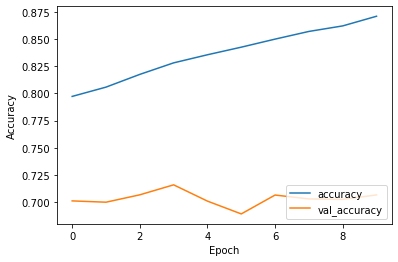
\includegraphics[width=0.4\textwidth]{img/model_surapprentissage_acc.png} }}
        \qquad
        \subfloat[Avec Dropout]{{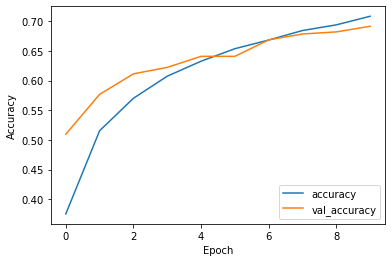
\includegraphics[width=0.4\textwidth]{img/model_dropout_acc.png} }}
    \end{figure}

\end{frame}



\begin{frame}{Amélioration de la structure}

\begin{block}<>{Élargir le modèle}<>
    \begin{description}
        \item[BatchNormalization] Ajout d'une couche de BatchNormalization après chaque couche de convolution ainsi que les couches denses.
        \item[Dense] Ajout d'une couche dense de 512 neurones.
    \end{description}
\end{block}

\begin{figure}
    \centering
    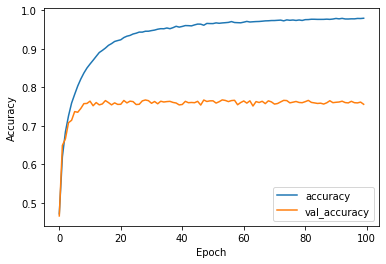
\includegraphics[width=0.5\textwidth]{img/Model1_without_dataug_acc.png}
    \caption{Évaluation après l'amélioration}
\end{figure}
\end{frame}


\section{Optimisation des résultats}
\placelogofalse
\begin{frame}{Data augmentation}
    \begin{itemize}
        \item Une rotation des images;
        \item Retourner l'image verticalement ou/et horizontalement;
        \item Décaler l'image de quelques pixels de droite à gauche ou/et de haut en bas.
    \end{itemize}
    \begin{figure}
        \centering
        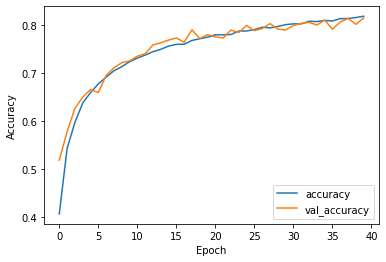
\includegraphics[width=0.5\textwidth]{img/with_data_aug_acc.png}
        \caption{Évaluation après data augmentation}
    \end{figure}
\end{frame}


\begin{frame}{Variation des hyperparamètres}
    \begin{block}<>{Best\_params}<>
        Ça consite à trouver les meilleurs hyperparamètres parmi :loss fonction, lerning rate, optimizer, dropout, pooling.
    \end{block}
    \begin{figure}
        \centering
        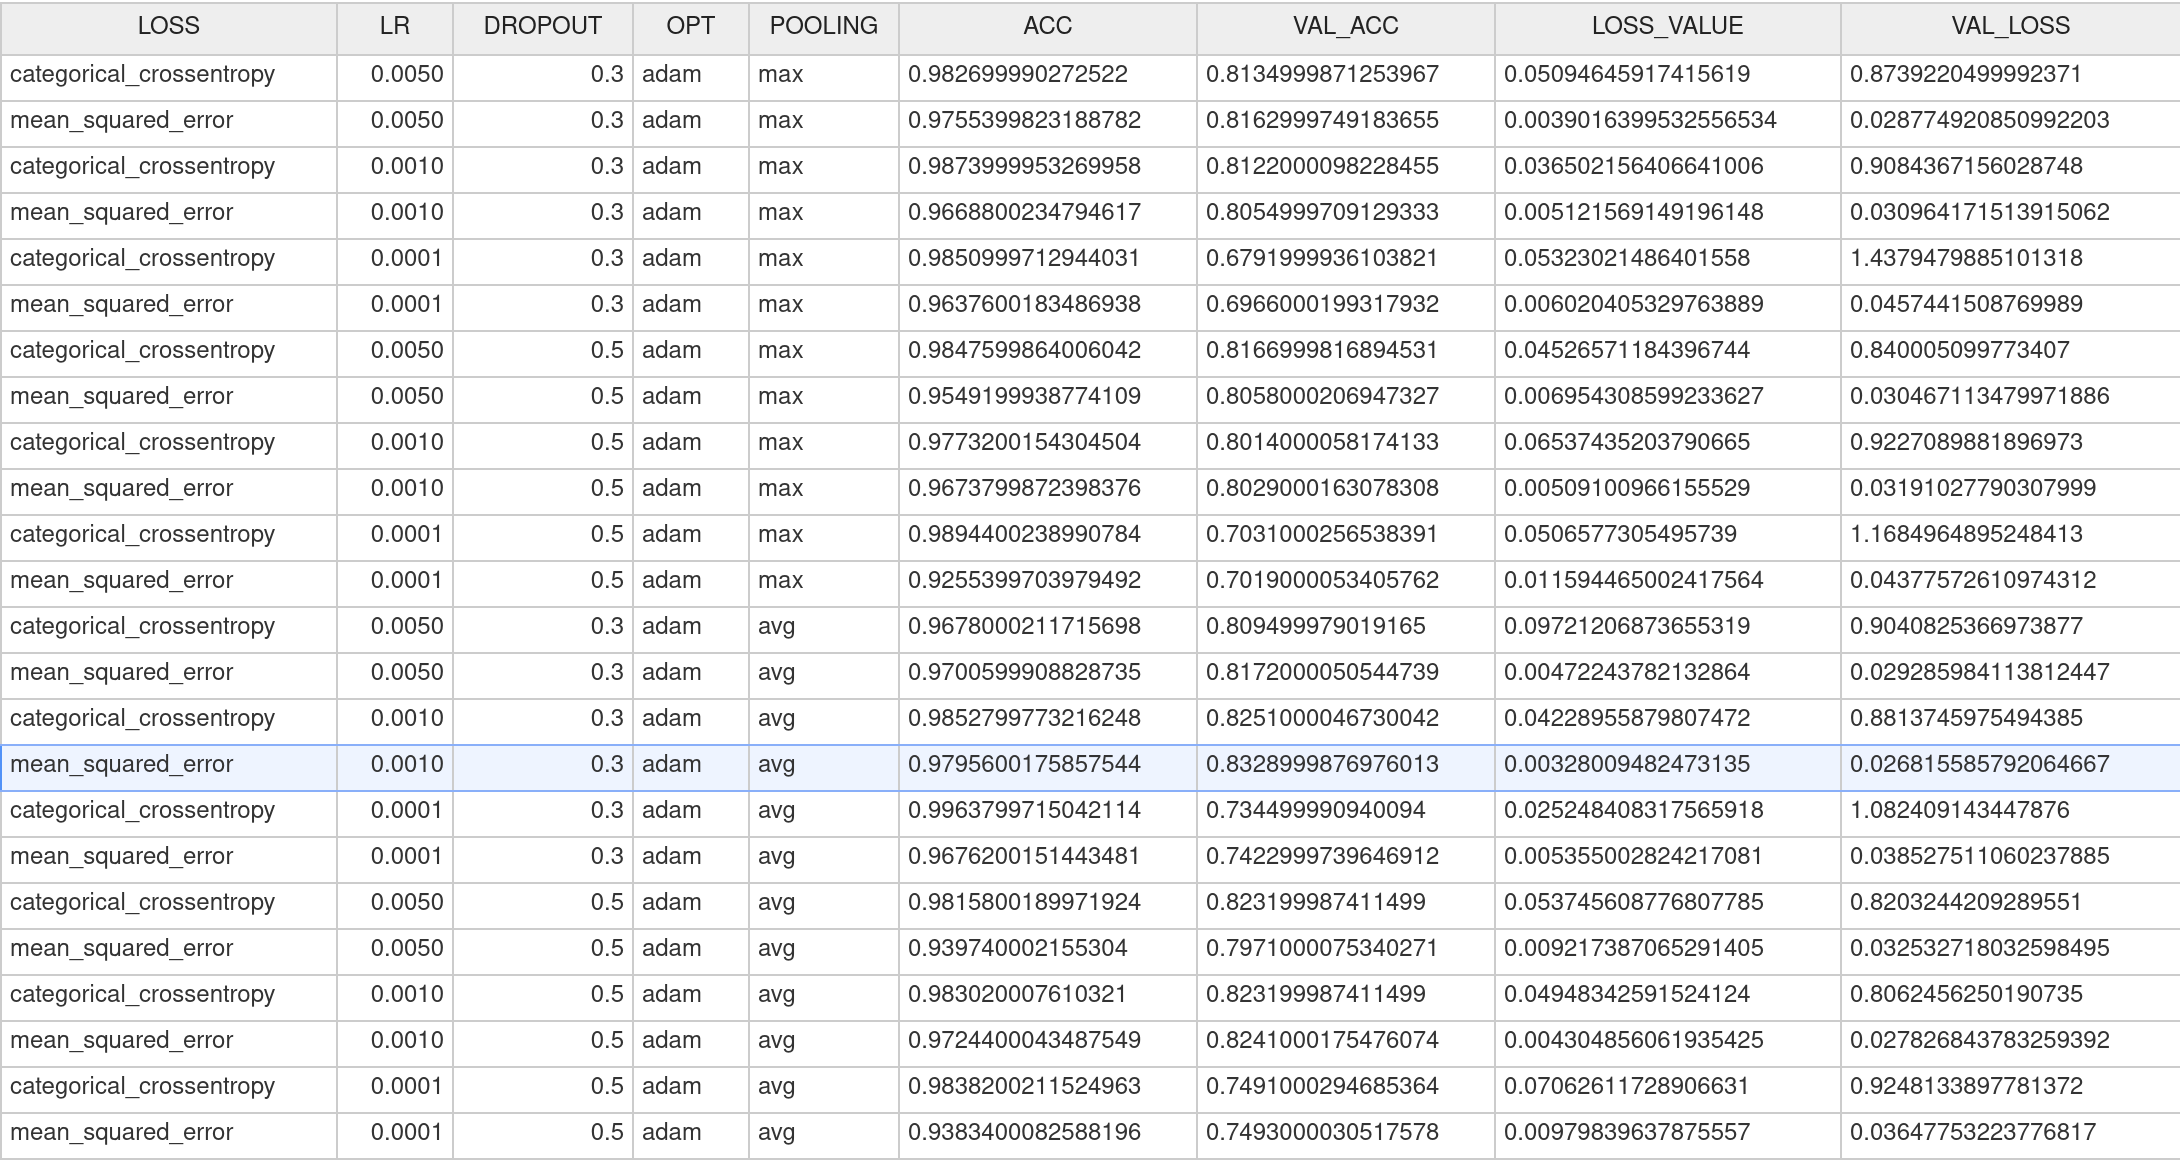
\includegraphics[width=0.7\textwidth]{img/csv.png}
        \caption{Tableau comparant les combinaison des hyperparamètres.}
    \end{figure}
\end{frame}

\begin{frame}{Dernière évaluation}
    \begin{figure}
        \centering
        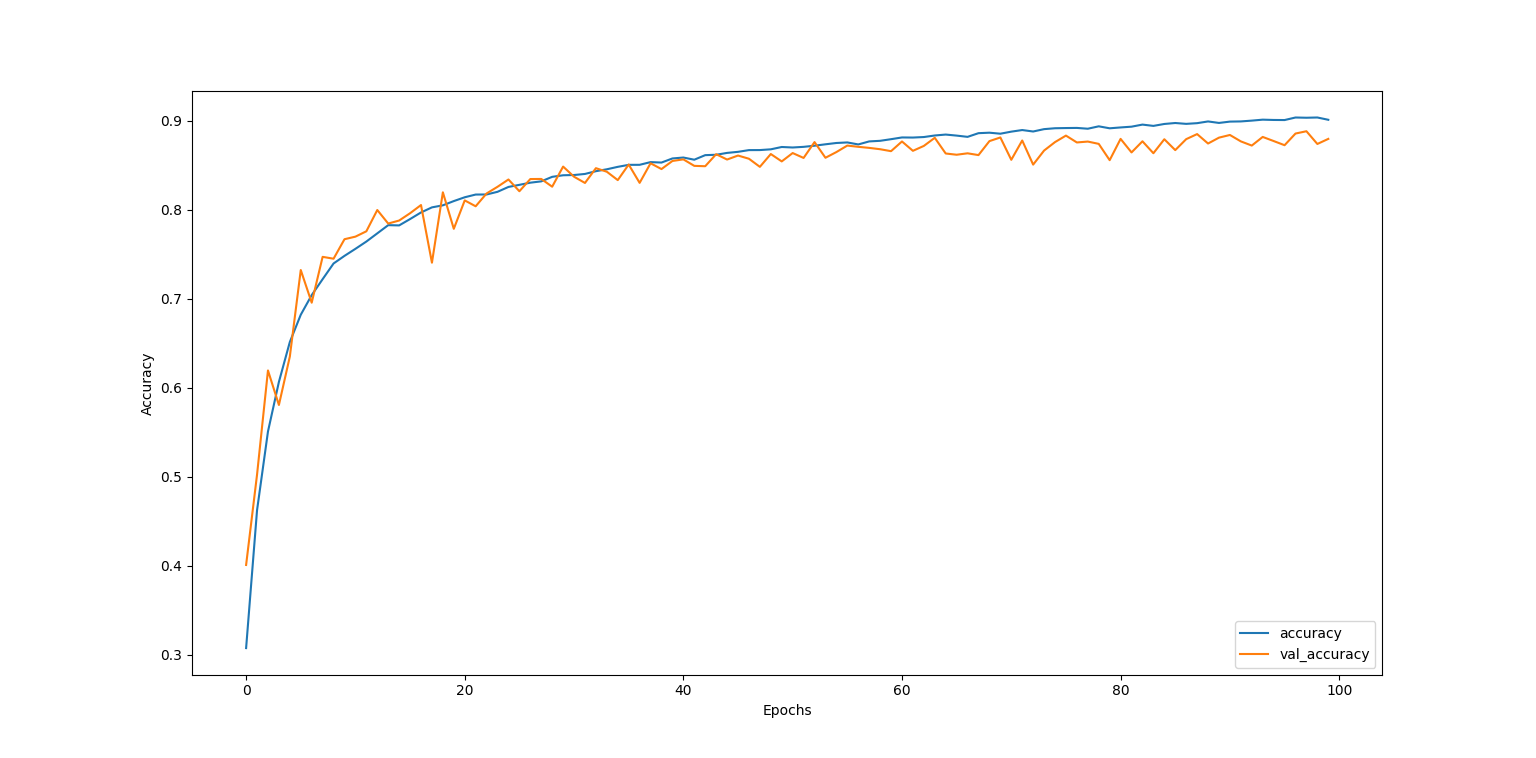
\includegraphics[width=0.9\textwidth]{img/model-final-acc.png}
        \caption{Évaluation après l'obtention des meilleurs hyperparamètres.}
    \end{figure}
\end{frame}


\section{Transfert learning}
\placelogofalse
\begin{frame}{modèles pré-entraînés}
    \begin{block}<>{}<>
        Choix de trois modèles pré-entraînés : 
        \begin{itemize}
            \item MobileNetV2.
            \item DenseNet121.
            \item VGG16.
        \end{itemize}
    \end{block}

    \begin{figure}
        \centering
        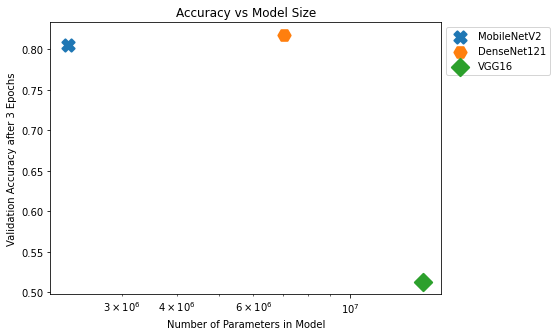
\includegraphics[width=0.6\textwidth]{img/index.png}
        \caption{Comparaison entre modèles pré-entraînés.}
    \end{figure}
\end{frame}

\begin{frame}{Comparaison des téchniques}
    \begin{block}{Transfert learning}
        Deux téchniques existe pour faire du transfert learning : 
        \begin{itemize}
            \item Feature Extraction.
            \item Fine tunning. 
        \end{itemize}
    \end{block}

    \begin{figure}
        \subfloat[Feature Extraction]{{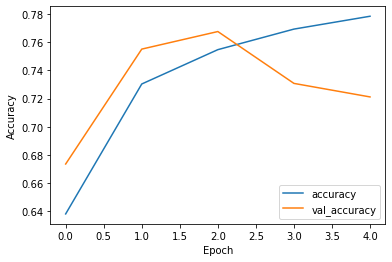
\includegraphics[width=0.4\textwidth]{img/ft_extraction/acc.png} }}
        \qquad
        \subfloat[Fine tunning]{{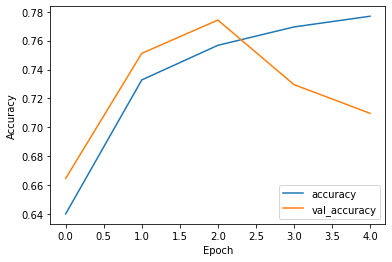
\includegraphics[width=0.4\textwidth]{img/fine_tunning/acc.png} }}
    \end{figure}

\end{frame}


\begin{frame}{Combinaison des téchniques}
    \begin{block}<>{}<>
        Par contre, il est possible de combiner les deux téchniques pour avoir un meilleur résultat.
    \end{block}

    \begin{figure}
        \centering
        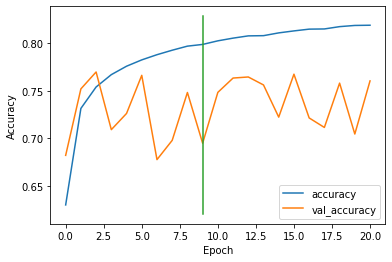
\includegraphics[width=0.6\textwidth]{img/combined_ft_extract_fine_tun/acc.png}
        \caption{Combinaison de Feature extraction avec du fine tunning.}
    \end{figure}

\end{frame}

\section{Conclusion et perspectives}

\begin{frame}{}
    \begin{block}<>{Atous du Projet}<>
        \begin{itemize}
            \item Data augmentation.
            \item Variation des hyperparamètres pour obtenir la meilleure combinaison de ces derniers.
            \item Transfert learning.
        \end{itemize}
    \end{block}
    \begin{block}<>{Perspectives}<>
        \begin{itemize}
            \item Varier plus d’hyperparamètres et d’options de data augmentation et pouvoir aussi les varier au
            même temps.
            \item Exploiter le transfert learning avec de la data augmentation.
        \end{itemize}
    \end{block}
\end{frame}


\begin{frame}{}
    \begin{center}
      Merci pour votre attention.
    \end{center}
\end{frame}
  
\end{document}